\documentclass[a4paper,12pt]{article} % тип документа
\usepackage[margin=1in]{geometry} % Поля

%  Русский язык
\usepackage[warn]{mathtext}
\usepackage[T2A]{fontenc}			% кодировка
\usepackage[utf8]{inputenc}			% кодировка исходного текста
\usepackage[english,russian]{babel}	% локализация и переносы
% Математика
\usepackage{amsmath,amsfonts,amssymb,amsthm,mathtools} 
\usepackage{wasysym}
%%%
\usepackage{graphicx}

\usepackage{tabularx}

\usepackage{gensymb} % знак градуса
\usepackage{enumitem} % изменить список enumerate
\usepackage{placeins} % \FloatBarrier

\renewcommand{\thesection}{\Roman{section}} 
\renewcommand{\thesubsection}{\roman{subsection}}



\begin{document} 
\begin{titlepage}
  \begin{center}
    \large
    Московский Физико-Технический Институт
    
    (Национальный исследовательский университет)
    \vspace{0.5cm}

   
    \vspace{0.25cm}
 
    \vfill
 
    \vfill

    \textsc{\bf{Лабораторная работа}}\\[5mm]
    
    {\LARGE Растровый электронный микроскоп и электронно-зондовый рентгеноспектральный микроанализ}
  \bigskip
    \vfill
    
\end{center}
\vfill
\begin{flushright}

    \textbf{Работу выполнили} \\
    Бичина Марина Андреевна \\
    Борток Даниил Евгеньевич \\
    Голощапов Михаил Юрьевич \\
    Давыдов Владислав Олегович \\
    Карташов Константин \\

\end{flushright}

\bigskip


\vfill

\begin{center}
  Долгопрудный, 2022 г.
\end{center}
\end{titlepage}

\section{Аннотация}

\subsection{Цель работы}

\paragraph{} Целью работы является знакомство с устройством растрового электронного микроскопа (РЭМ) и с физическими принципами его функционирования, и дальнейшее исследование нескольких образцов в различных режимах работы, а именно:
\begin{itemize}
\itemsep0em
\item Режим сбора истинно вторичных электронов (SE)
\item Режим сбора упруго отражённых электронов (BSE): топографический и элементный контрасты
\item Режим рассмотрения одного образца под разными углами
\item Режим рентгеноспектрального микроанализа.
\end{itemize}




\section{Задание}

\subsection{Изображение биологического объекта}

\paragraph{} Рассмотрим в электронном микроскопе крыло бабочки (рис. \ref{fig:butter}). В $1200\times$ кратном увеличении (а, б) видим, что чешуйки на крыле имеет зубчатые края и сетчатую микроструктуру. Для того чтобы различить более тонкие структуры рассмотрим крыло в $8000\times$ (в) и $7000\times$ (г) кратном увеличении. Видим, что микроструктура крыла представляет из себя сеточку из ячеек с характерными размерами порядка $l \sim 1.2\div0.4$ мкм, что примерно соответствует длине видимого света. Этим в частности объясняется "переливающийся" окрас крыльев бабочки, и почему из крыльев бабочек нельзя создать краситель (при физическом и химическом воздействии разрушается микроструктура крыла).

\begin{figure}[h]
\centering
\begin{minipage}{0.49\textwidth}
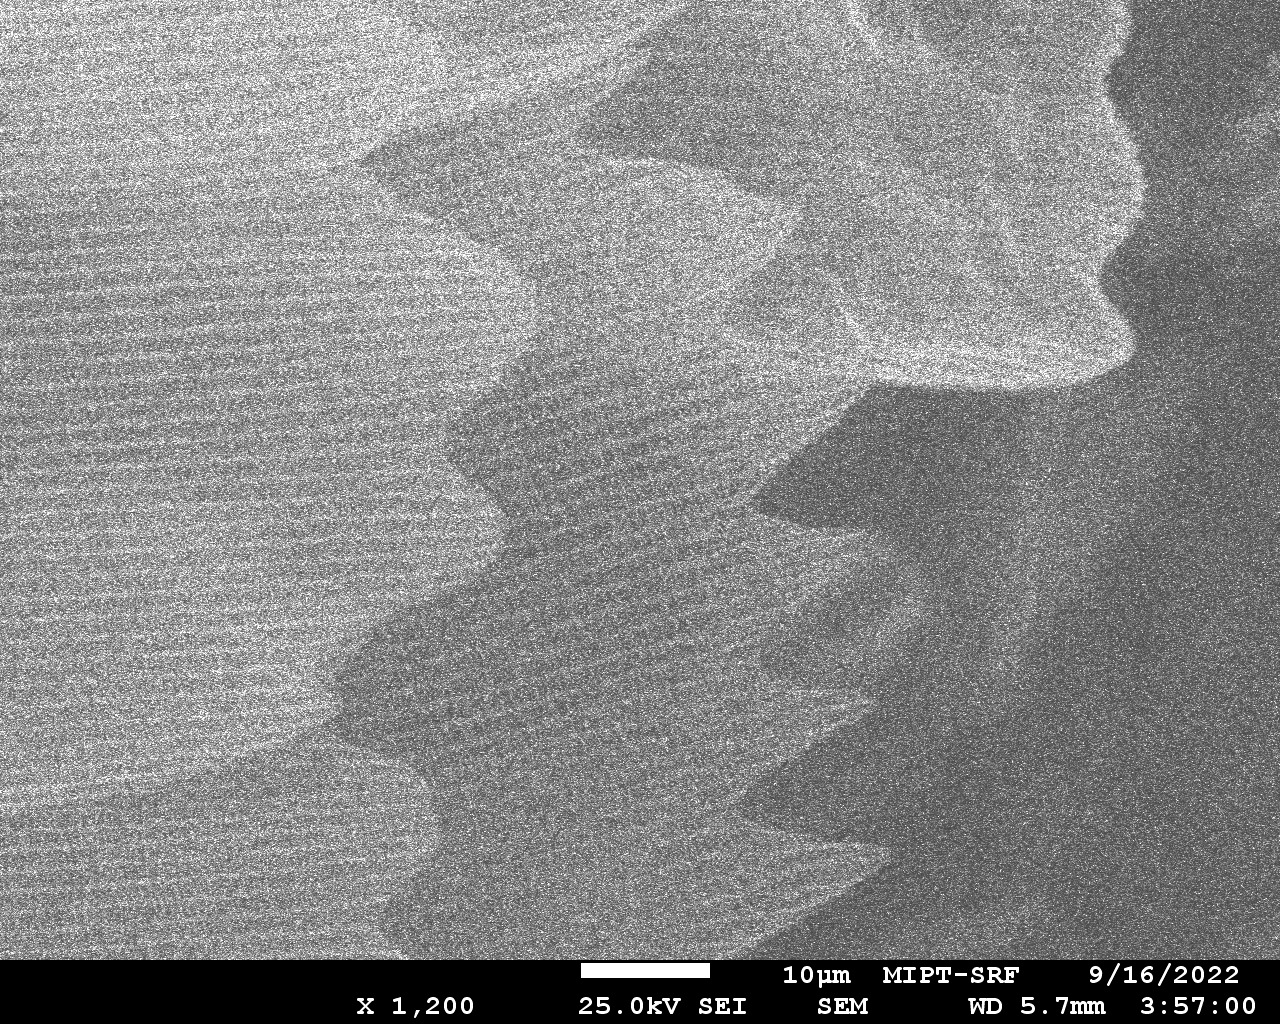
\includegraphics[width=\textwidth]{Butterfly001.jpg}
\vspace{-2em}
\center{(а)}
\end{minipage}
\begin{minipage}{0.49\textwidth}
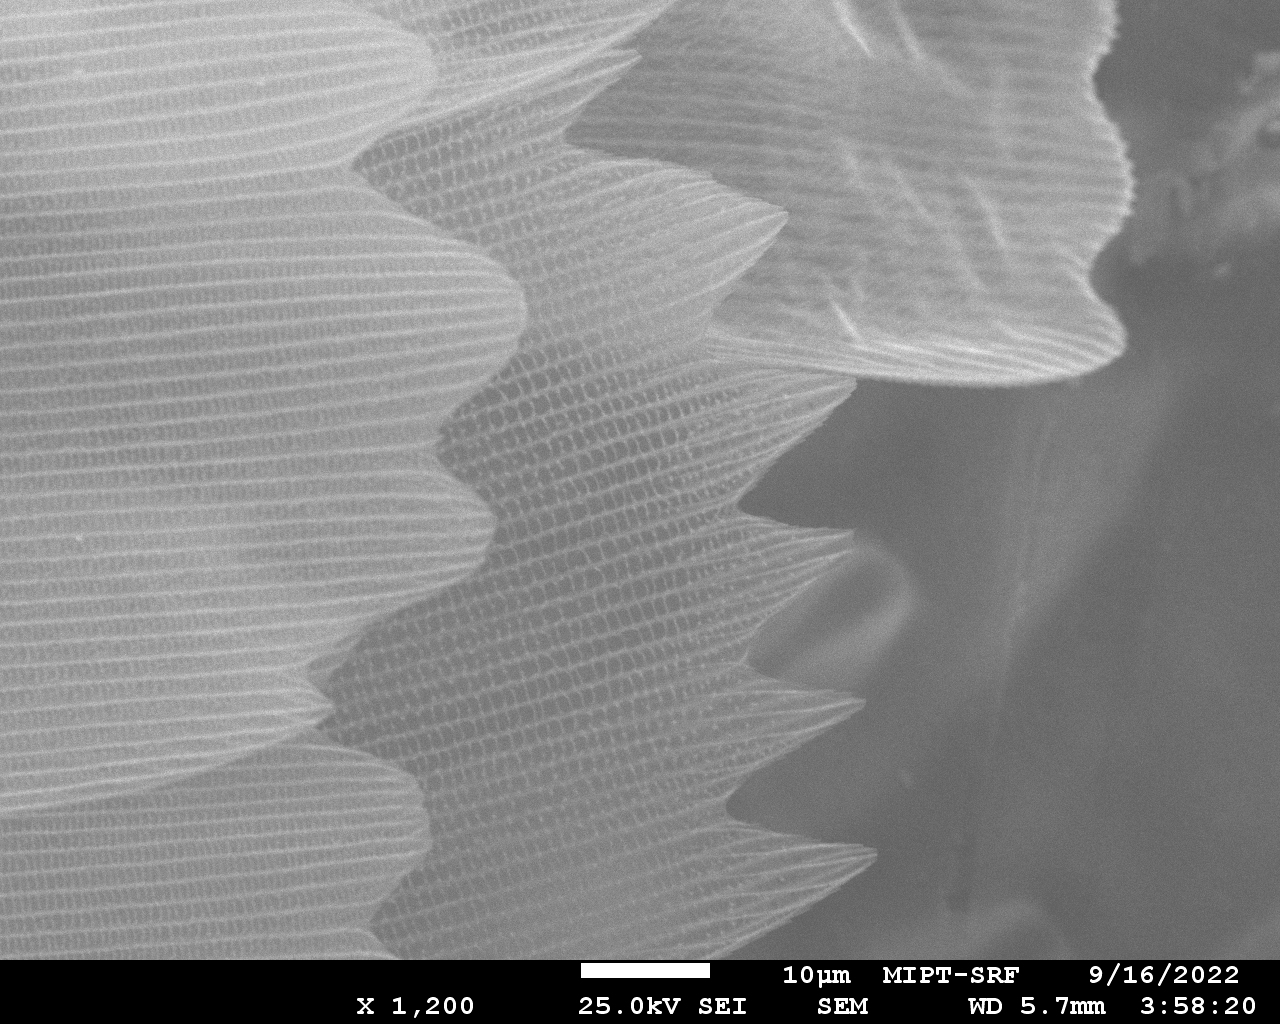
\includegraphics[width=\textwidth]{Butterfly002.jpg}
\vspace{-2em}
\center{(б)}
\end{minipage}
\begin{minipage}{0.49\textwidth}
\vspace{0.5em}
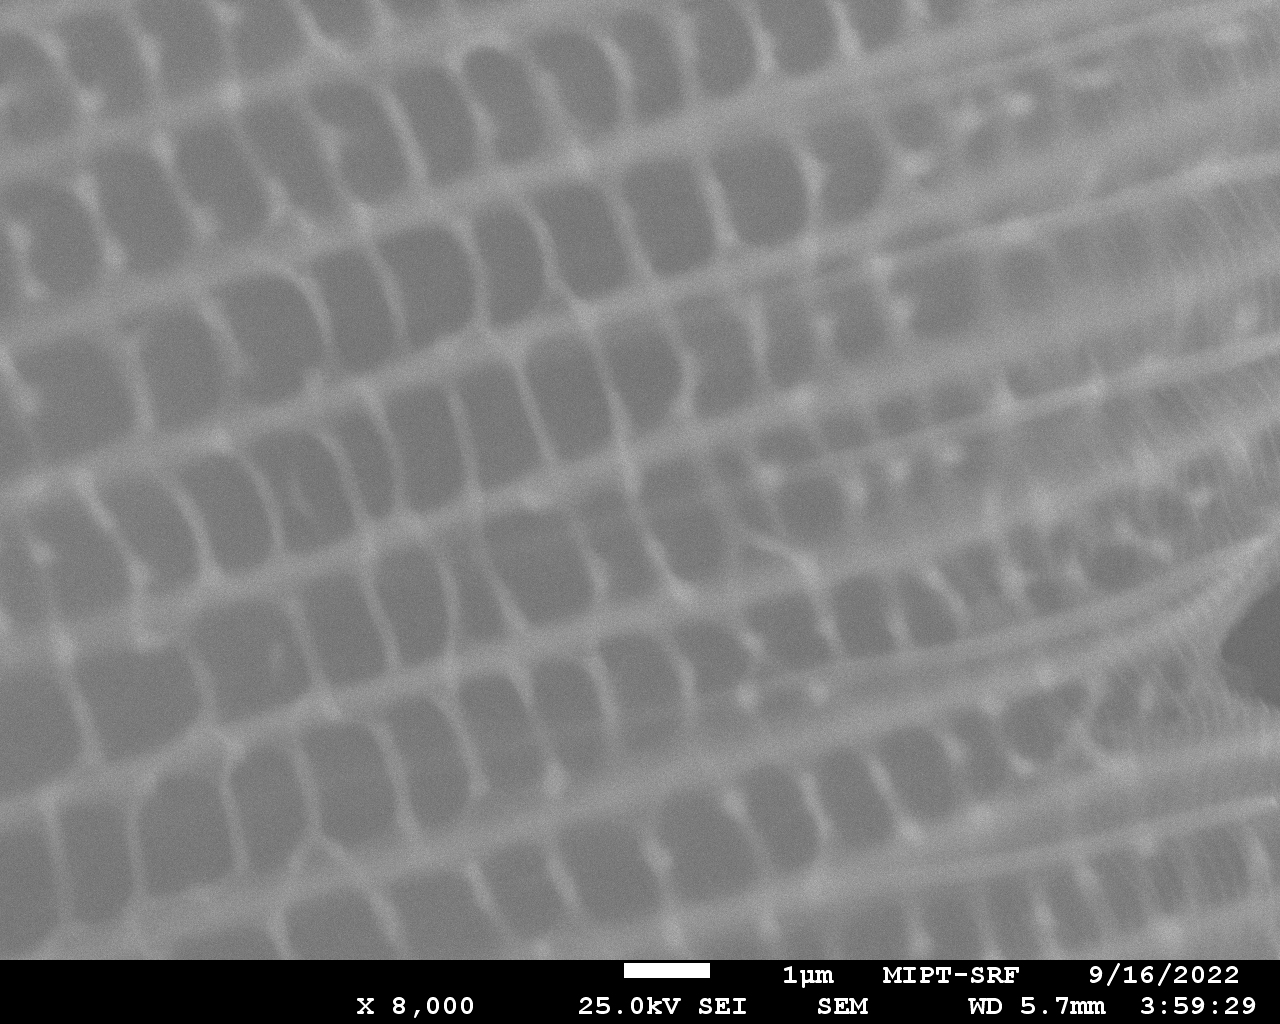
\includegraphics[width=\textwidth]{Butterfly003.jpg}
\vspace{-2em}
\center{(в)}
\end{minipage}
\begin{minipage}{0.49\textwidth}
\vspace{0.5em}
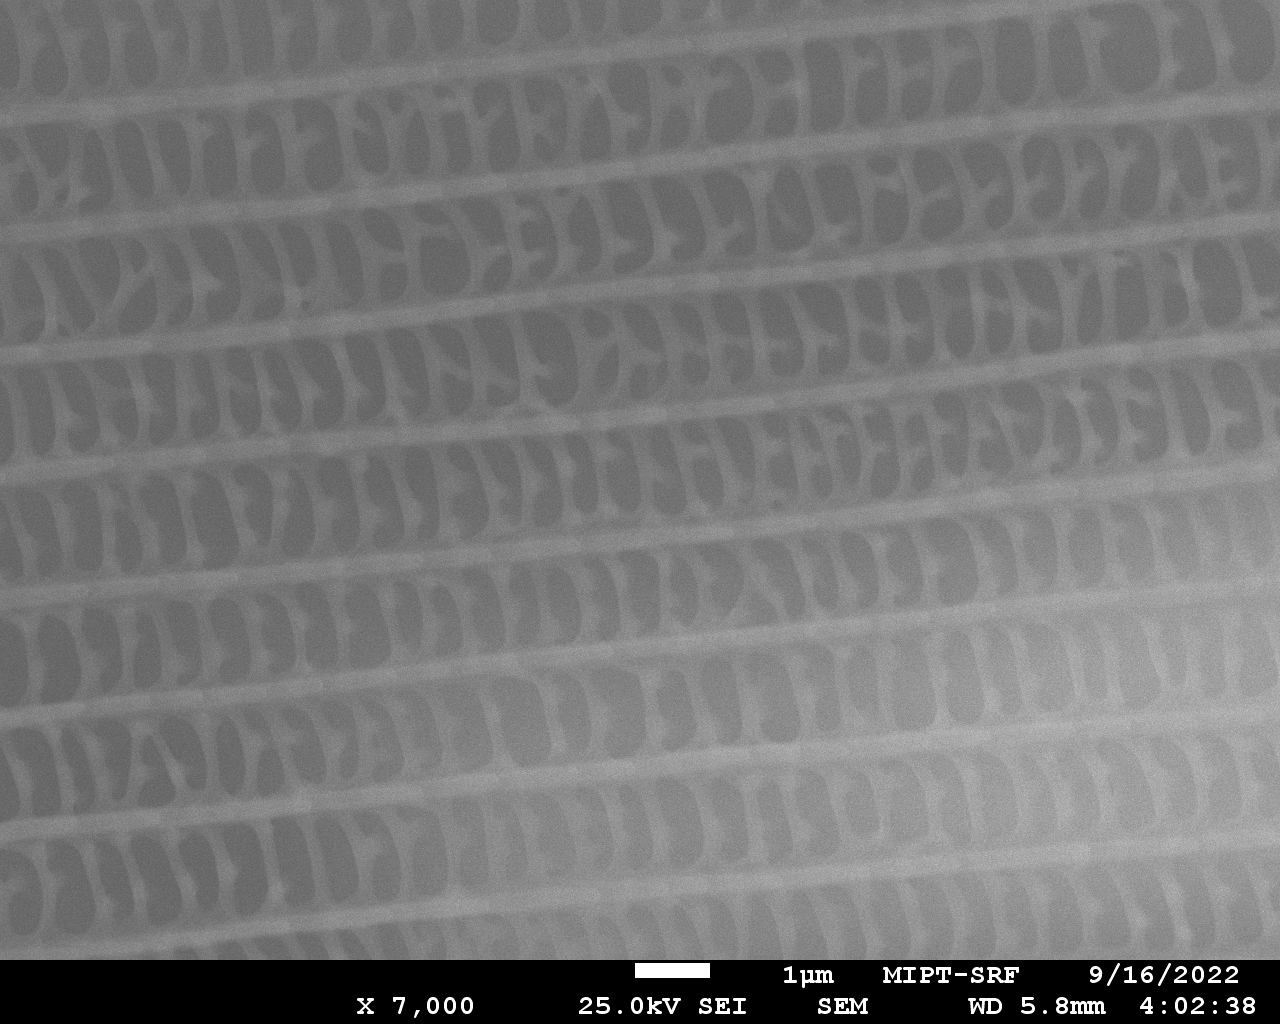
\includegraphics[width=\textwidth]{Butterfly004.jpg}
\vspace{-2em}
\center{(г)}
\end{minipage}
\caption{Полученные изображения крыла бабочки}
\label{fig:butter}
\end{figure}

\subsection{Изображение образца медь--хром}
\label{sus}

\paragraph{} Рассмотрим под различными режимами работы РЭМ образец медь--хром представляющий собой таблетку из сплава меди и хрома (рис \ref{fig:tablet}). 

Для начала рассмотрим образец при режиме сбора истинно вторичных электронов (а). Видим рельеф образца в достаточно подробных деталях: видные две большие царапины, а также много менее глубоких царапин. Если присмотреться можно увидеть, что на образце есть области в которых царапины менее глубокие, чем в остальных. Разумно предположить, что в этих областях образец состоит из хрома, так как хром более твёрдый металл, чем медь. 

Далее рассмотрим образец в режиме сбора упруго отражённых электронов в элементном контрасте (б). Теперь рельеф образца практически не различим, но при этом видны обрасти разной яркости. Области с большей яркостью соответствуют областями образца состоящим из более тяжёлого элемента, то есть меди. Области с меньшей яркостью соответственно -- из хрома. Видим, что полученный результат подтверждает предыдущее предположение о составе образца.

Под конец рассмотрим образец в том же режиме в топографическом контрасте (в). Снова видим рельеф, при этом с большей контрастностью чем в (а), но при этом детальность изображения значительно меньше.


\begin{figure}[h]
\centering
\begin{minipage}{0.49\textwidth}
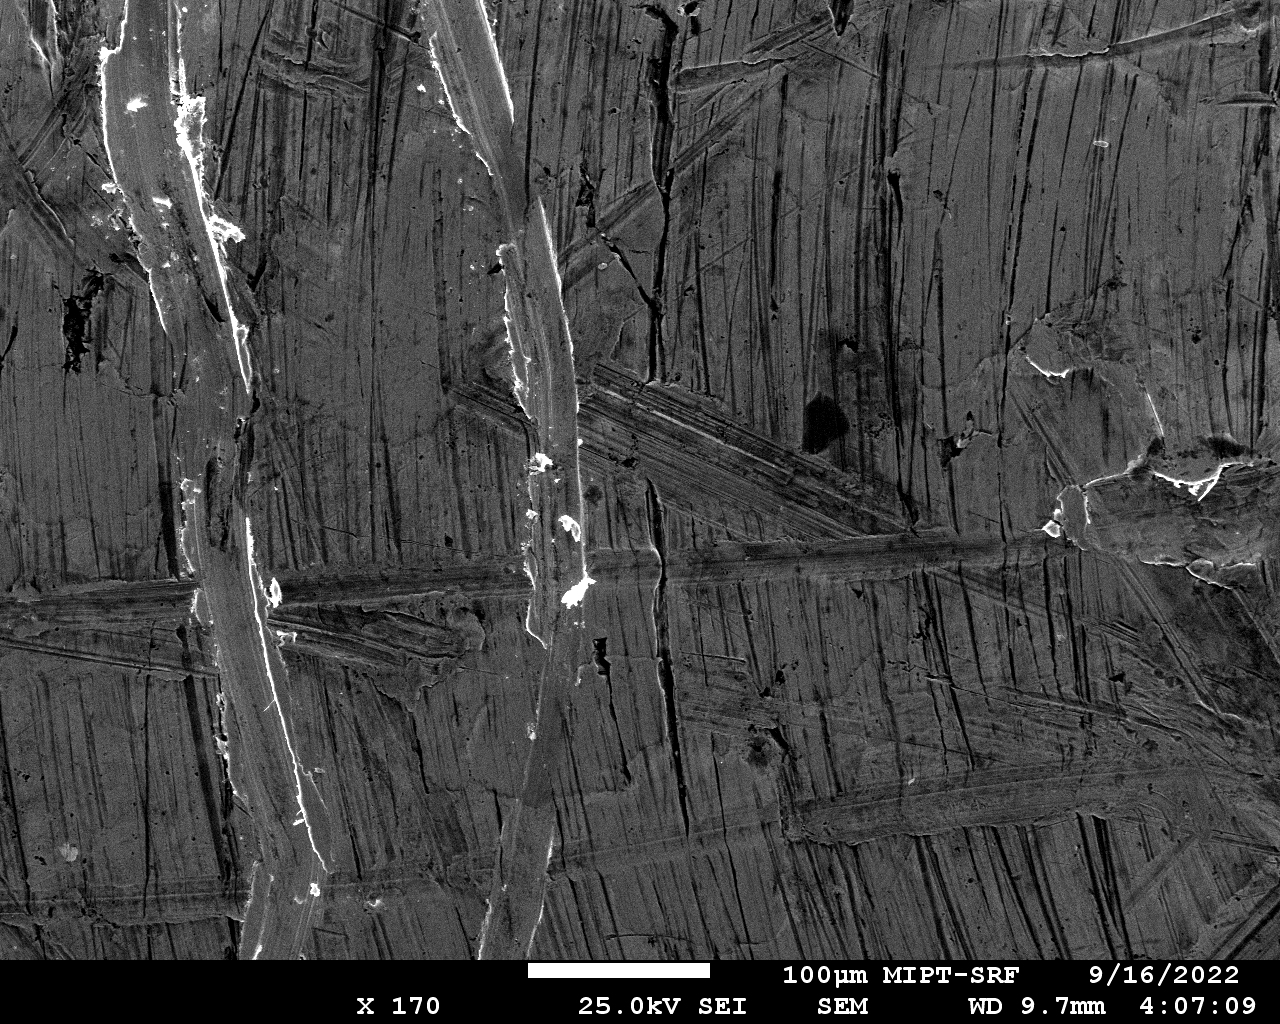
\includegraphics[width=\textwidth]{Tablet002.jpg}
\vspace{-2em}
\center{(а) SE}
\end{minipage}
\begin{minipage}{0.49\textwidth}
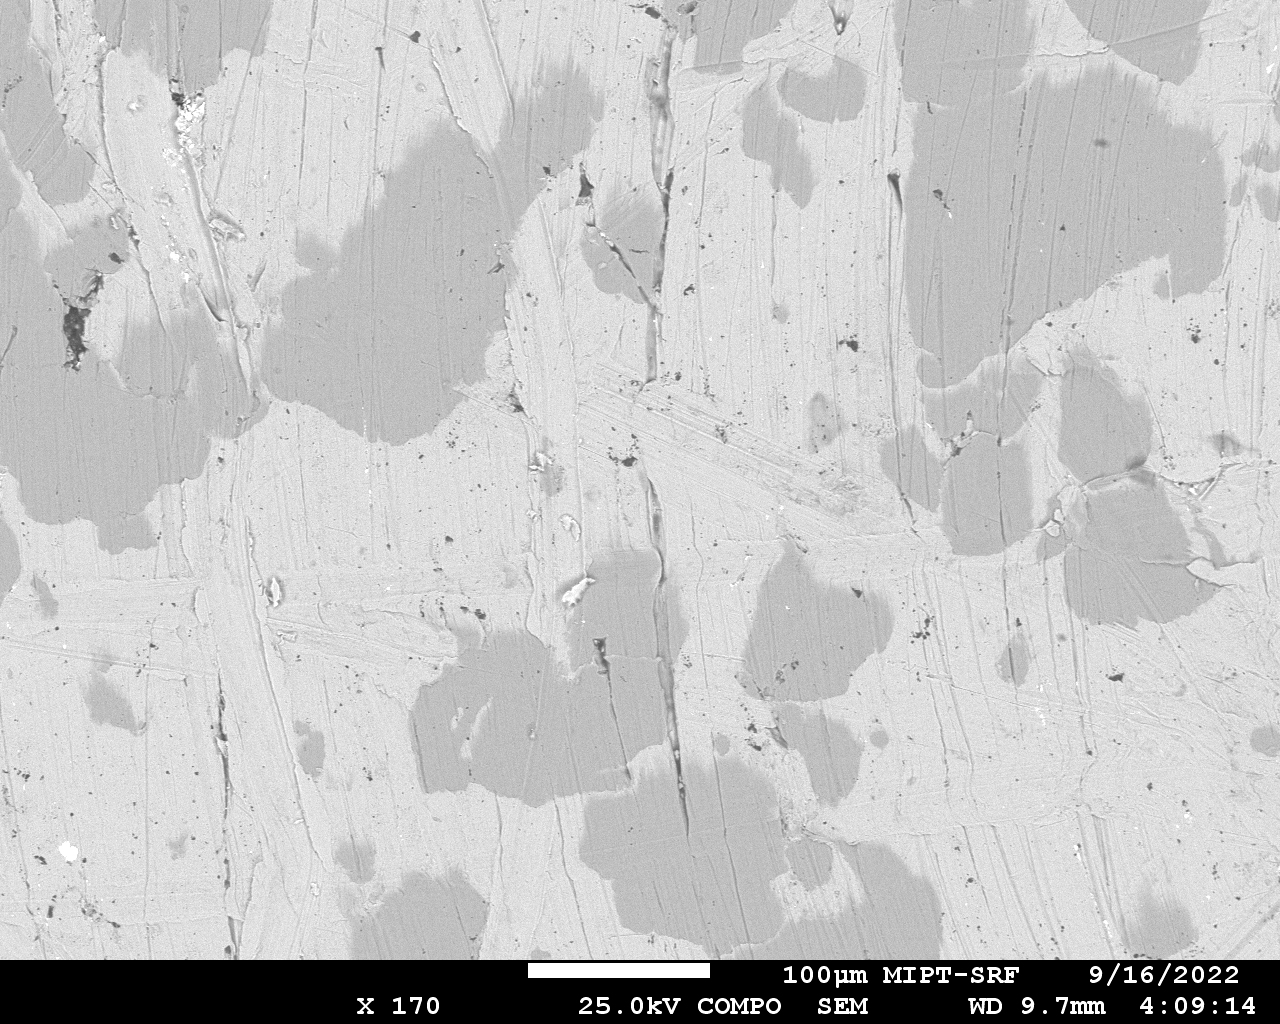
\includegraphics[width=\textwidth]{Tablet003.jpg}
\vspace{-2em}
\center{(б) BSE элементный контраст} 
\end{minipage}
\begin{minipage}{0.49\textwidth}
\vspace{0.5em}
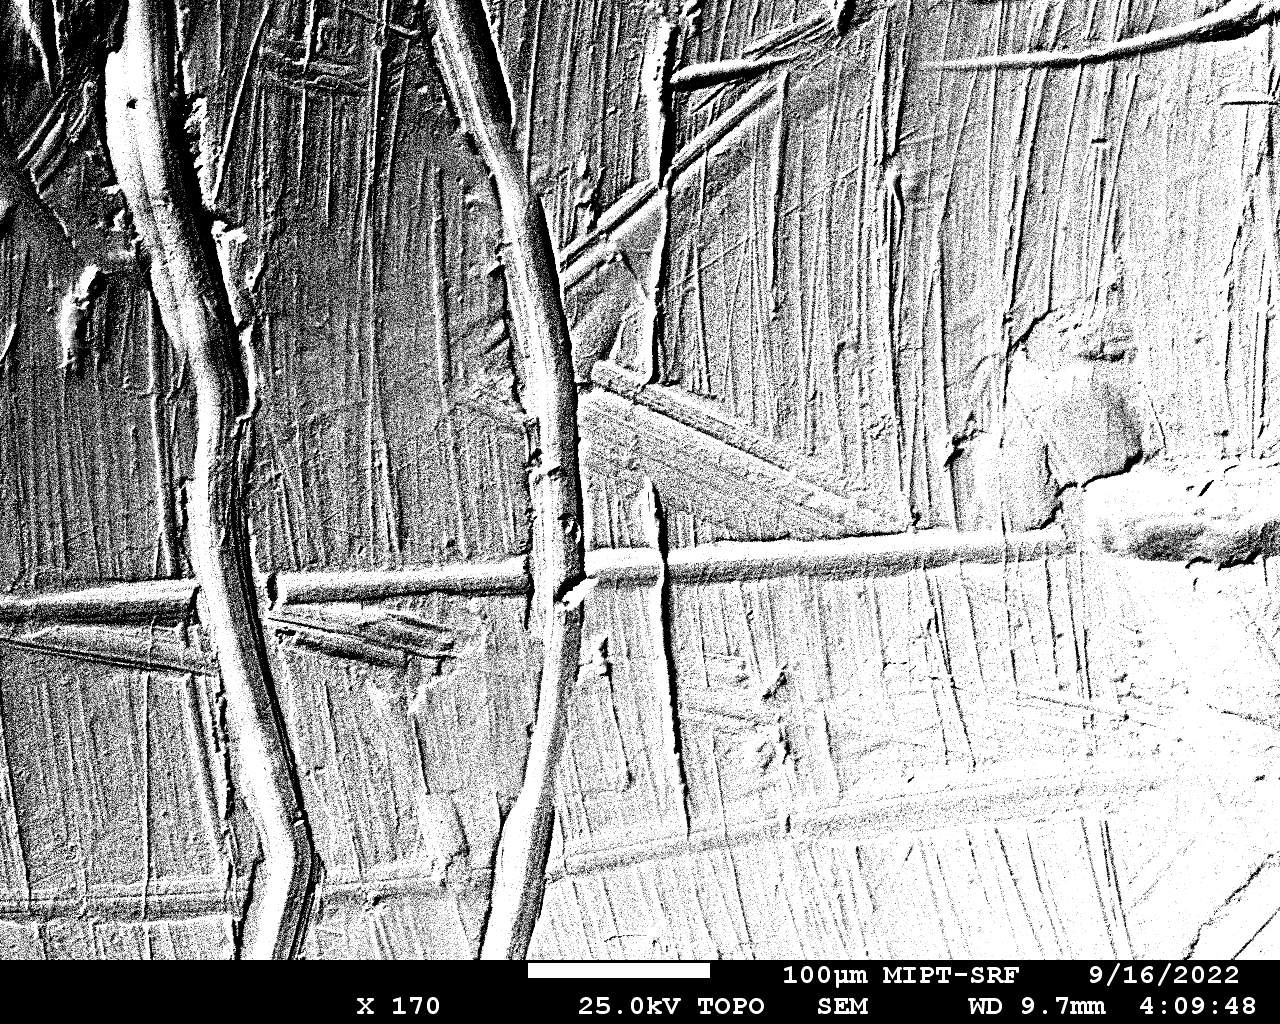
\includegraphics[width=\textwidth]{Tablet004.jpg}
\vspace{-2em}
\center{(в) BSE топографический контраст}
\end{minipage}

\caption{Изображения образца медь-хром снятые в различных режимах работы РЭМ}
\label{fig:tablet}
\end{figure}

\subsection{Микроанализ образца медь-хром}

\paragraph{} Переключим РЭМ в режим рентгеноспектрального микроанализа. Найдём, используя элементный контраст (рис. \ref{fig:comp}a), участок образца на котором виды области из меди и из хрома. 

Далее найдём рентгеновский спектр этого участка (рис. \ref{fig:plot}). Видим, что на спектре, как и ожидалось, присутствуют пики соответствующие хрому и меди. Также видны пики соответствующие углероду и кислороду, что неудивительно, учитывая то, что перед помещением образца в камеру микроскопа, он никак не очищался (виден рентгеновский спектр органических загрязнений). 

Составим элементные карты образца (рис. \ref{fig:comp}). В качестве референса используем элементный контраст (а). Рассмотрим элементные карту меди (б) и хрома (в): видим, что распределение меди и хрома совпадает предположенными в п.\ref{sus} распределением. На элементной карте углерода (г) не заметны какие-либо закономерности, разумно предположить, что органические загрязнения распределены равномерно по поверхности образца. На элементной карте кислорода (д) видна большая плотность в областях, в которых образец состоит из хрома, видимо хром сильнее взаимодействует с кислородом, чем медь.


\begin{figure}[h]
\centering
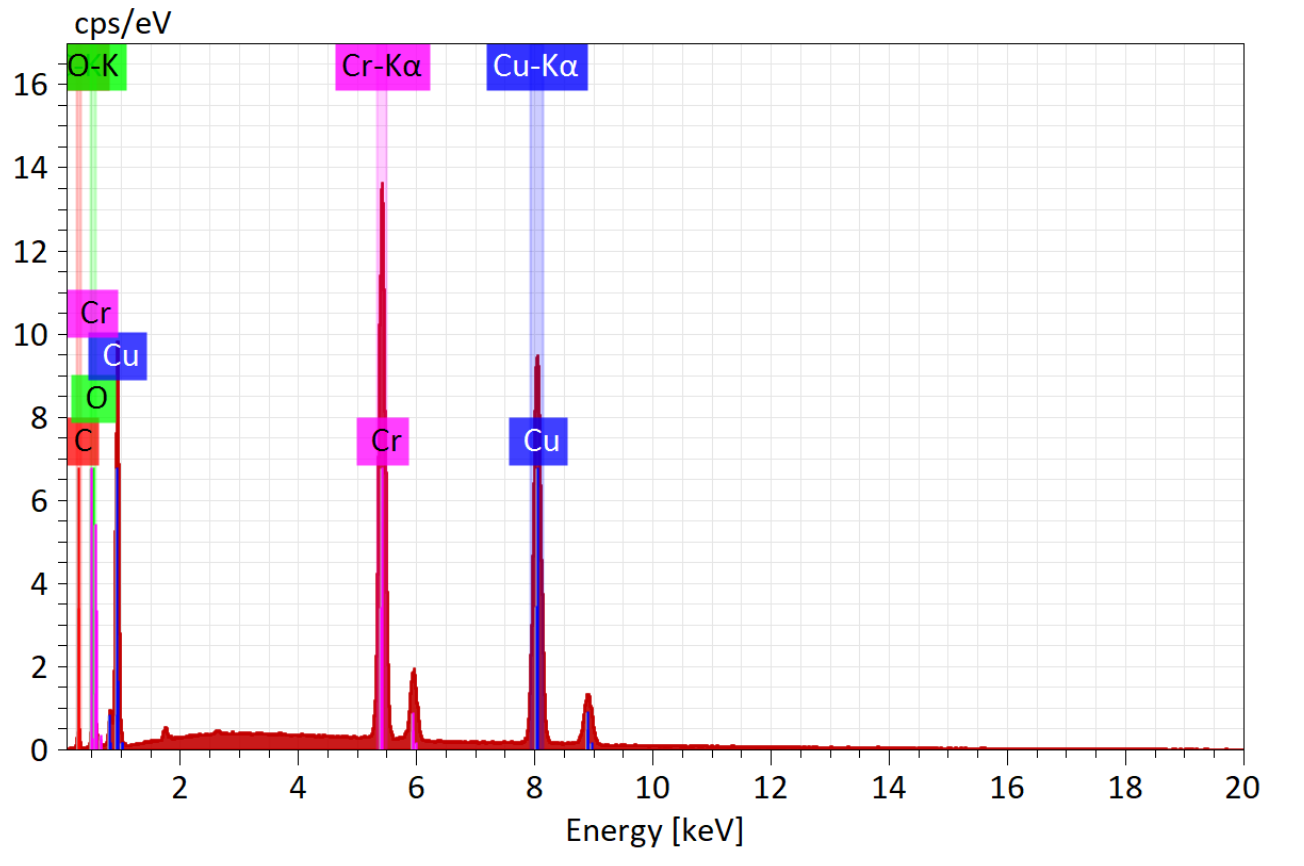
\includegraphics[width=\textwidth]{spectrum_plot.png}
\caption{Рентгеновский спектр образца}
\label{fig:plot}
\end{figure}


\begin{figure}[h]
\centering
\begin{minipage}{0.49\textwidth}
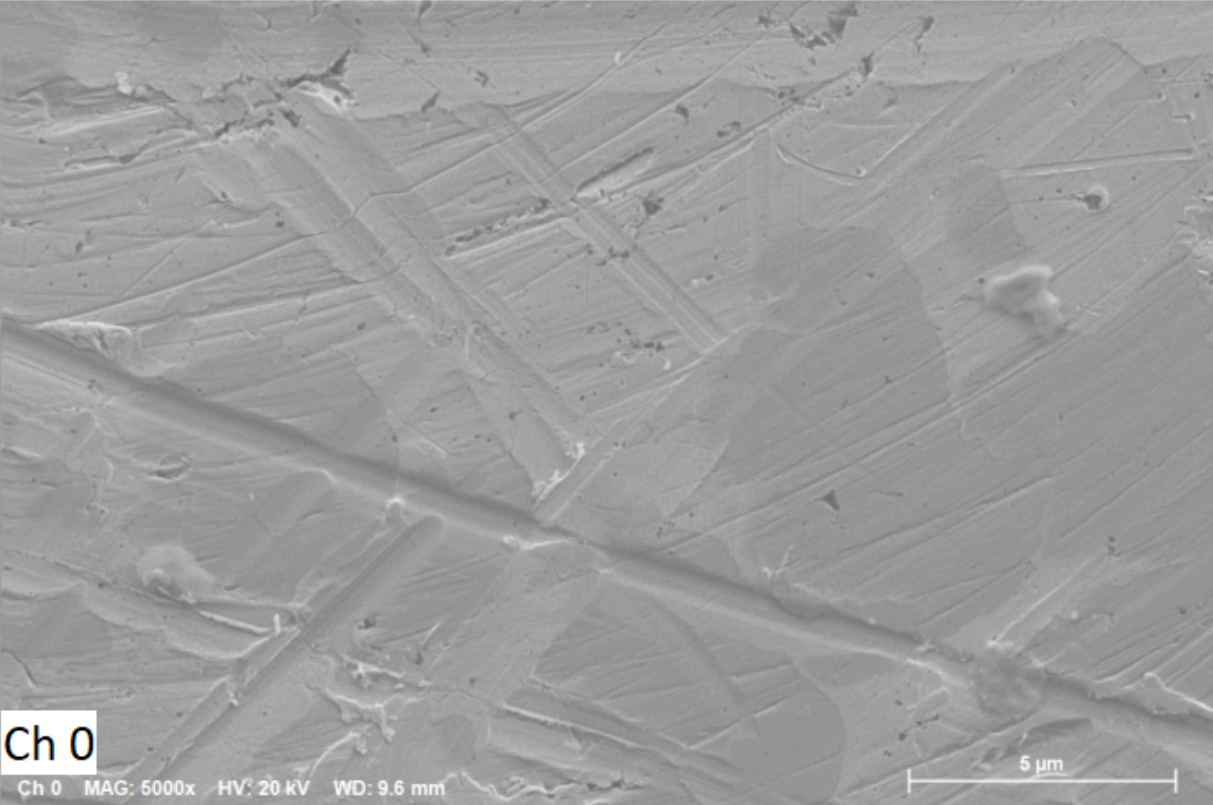
\includegraphics[width=\textwidth]{spectrum_0.png}
\vspace{-2em}
\center{(а) BSE элементный контраст}
\end{minipage}
\begin{minipage}{0.49\textwidth}
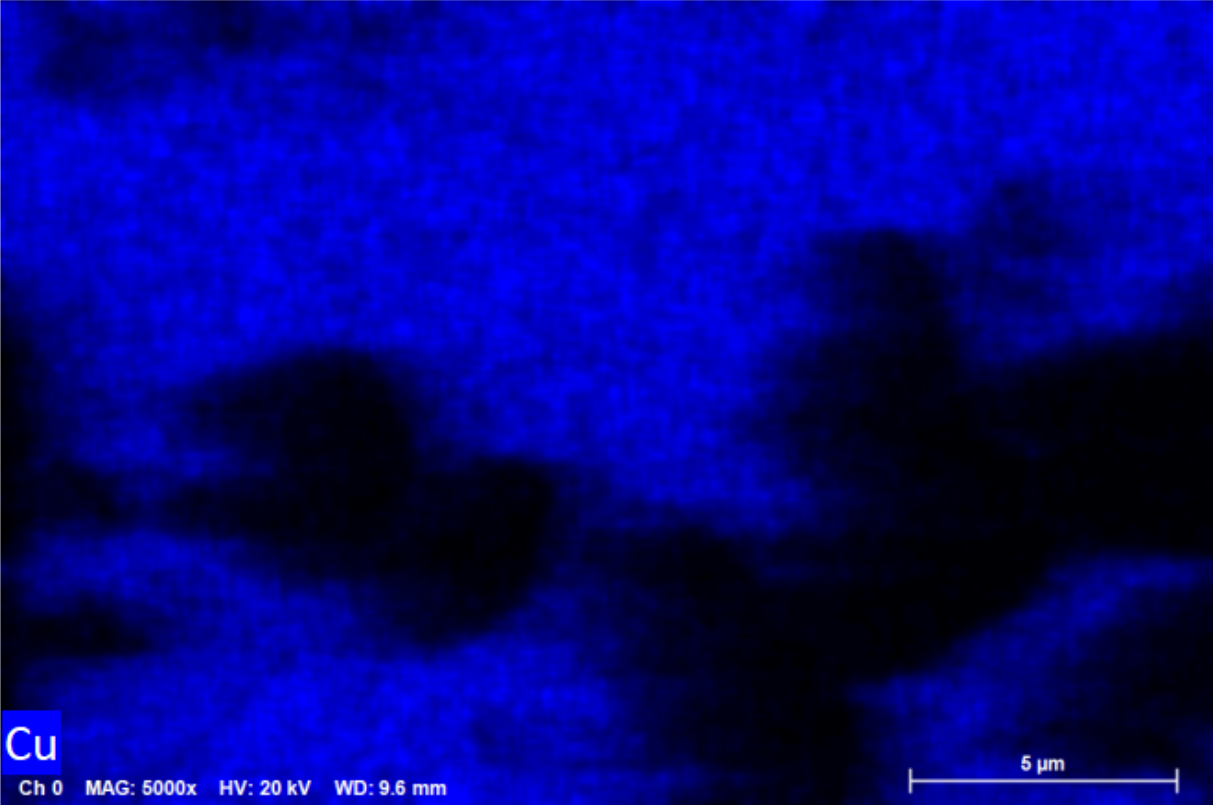
\includegraphics[width=\textwidth]{spectrum_cu.png}
\vspace{-2em}
\center{(б) элементная карта меди} 
\end{minipage}
\begin{minipage}{0.49\textwidth}
\vspace{0.5em}
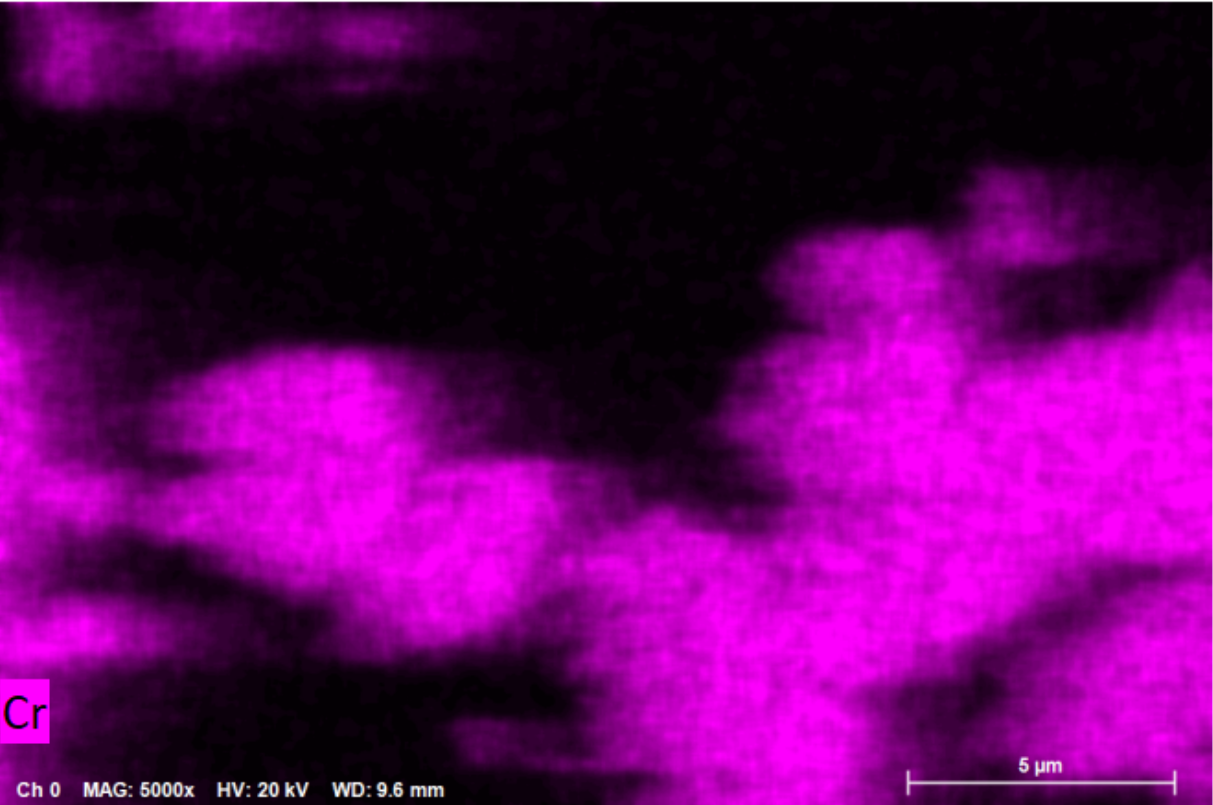
\includegraphics[width=\textwidth]{spectrum_cr.png}
\vspace{-2em}
\center{(в) элементная карта хрома}
\end{minipage}
\begin{minipage}{0.49\textwidth}
\vspace{0.5em}
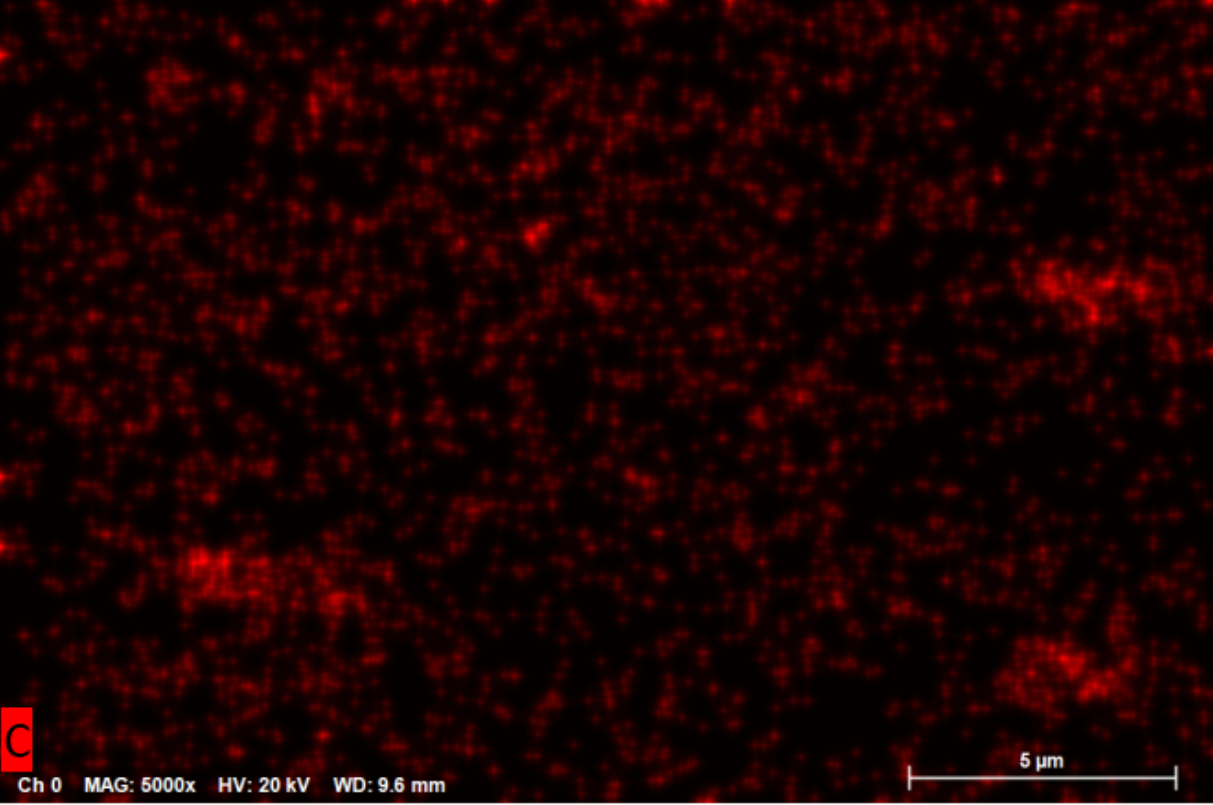
\includegraphics[width=\textwidth]{spectrum_c.png}
\vspace{-2em}
\center{(г) элементная карта углерода} 
\end{minipage}
\begin{minipage}{0.49\textwidth}
\vspace{0.5em}
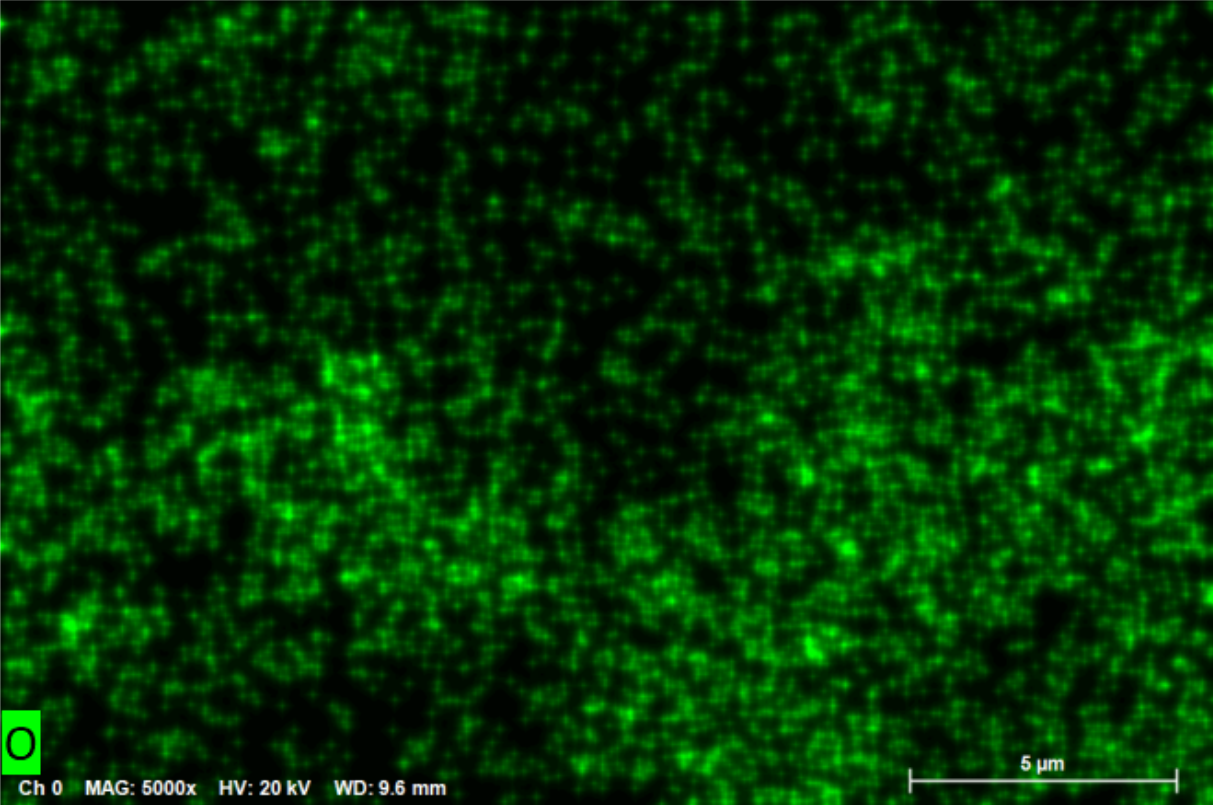
\includegraphics[width=\textwidth]{spectrum_o.png}
\vspace{-2em}
\center{(д) элементная карта кислорода}
\end{minipage}

\caption{Элементные карты образца}
\label{fig:comp}
\end{figure}

\subsection{Каналирование}

\paragraph{} Рассмотрим под РЭМ два образца из монокристалла кремния с кубической кристаллической решёткой (рис. \ref{fig:si}). 

На изображении (а) видны две перпендикулярные тонкие полосы и две перпендикулярные толстые полосы расположенные под углом $45\degree$ к тонким. Из соображений симметрии можно заключить, что в этом образце видна плоскость $(1,0,0)$ кристаллической решётки. 

На изображении (b) видны три тонкие полосы под углами $60\degree$ друг к другу. Также заметные три толстые полосы  $60\degree$ друг к другу и под углом $30\degree$ к тонким. Для этого образца можно заключить, что в нём видна плоскость $(1,1,1)$ кристаллической решётки.  

\begin{figure}[h]
\centering
\begin{minipage}{0.49\textwidth}
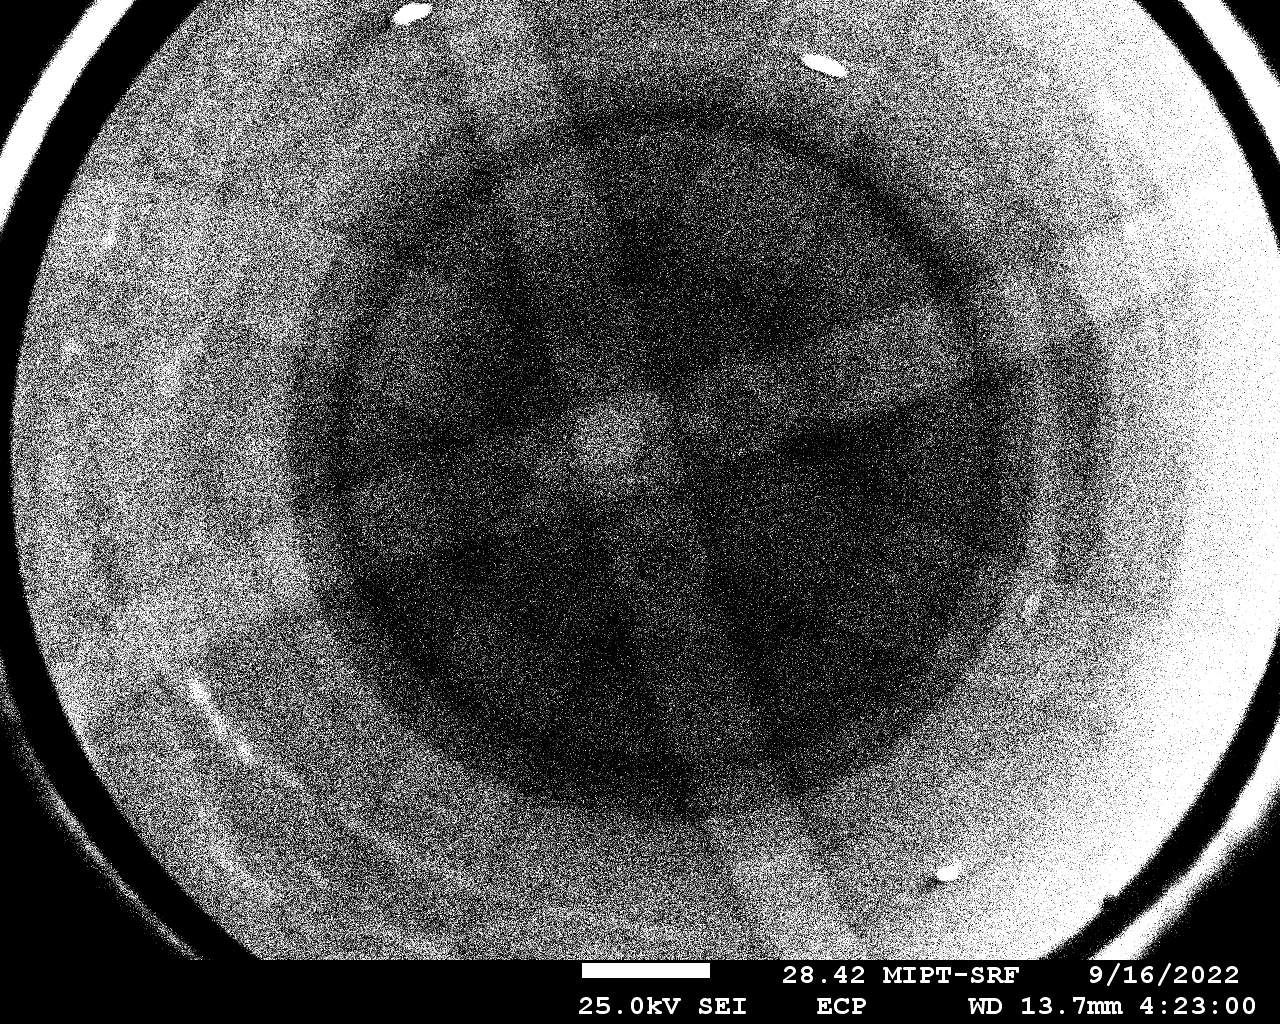
\includegraphics[width=\textwidth]{Si005.jpg}
\vspace{-2em}
\center{(а)}
\end{minipage}
\begin{minipage}{0.49\textwidth}
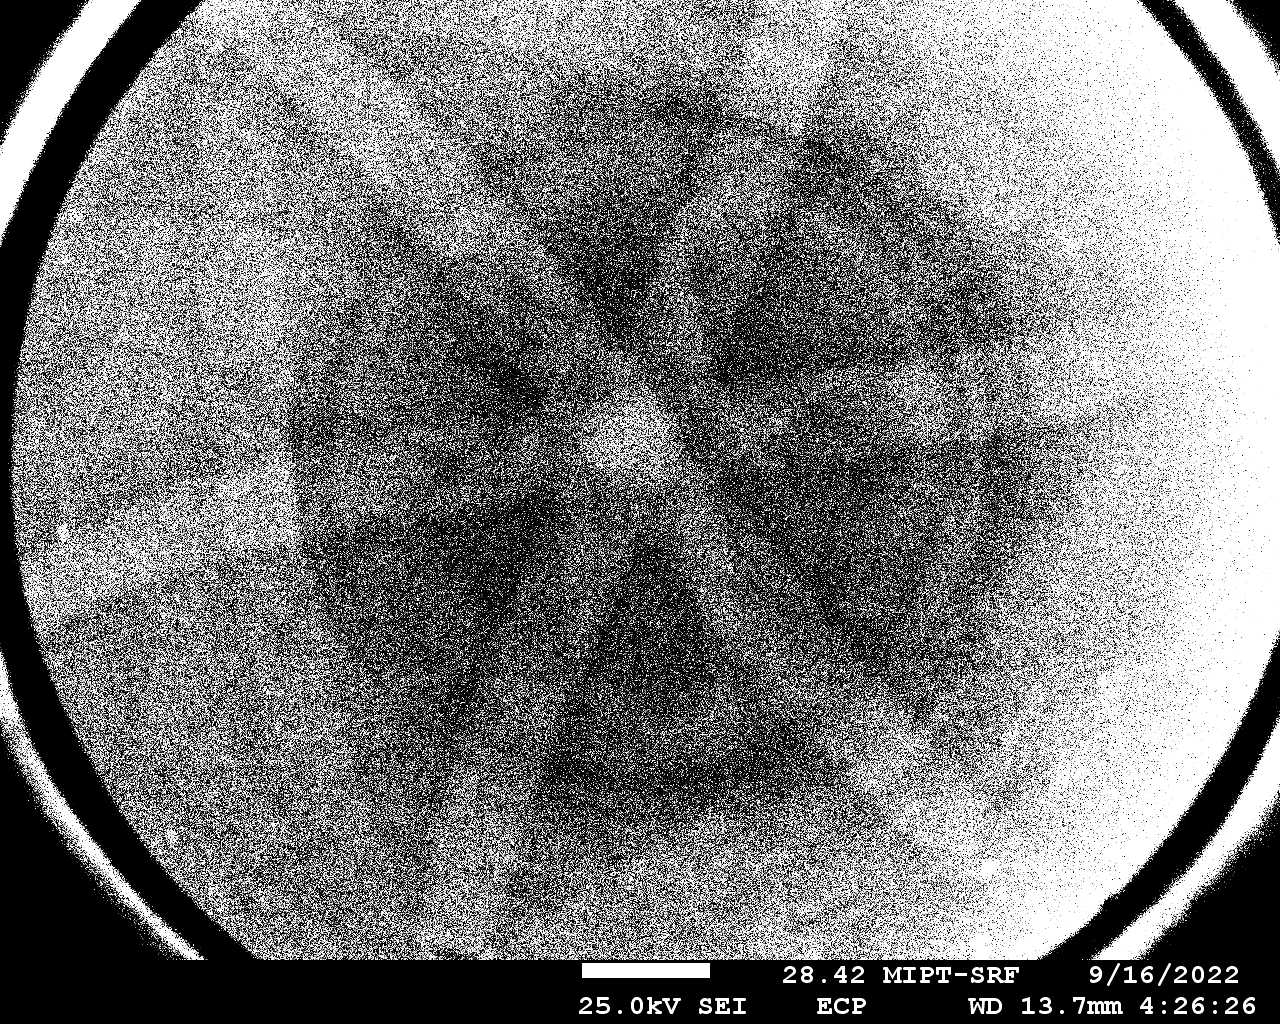
\includegraphics[width=\textwidth]{Si006.jpg}
\vspace{-2em}
\center{(б)}
\end{minipage}

\caption{Изображения двух образцов кремния сделанные в режиме каналирования}
\label{fig:si}
\end{figure}

\subsection{Зарядка диэлектрического образца}

\paragraph{} Рассмотрим под РЭМ образец из пенопласта (рис. \ref{fig:reflect}). Смотря на постоянно обновляющееся изображение на экране компьютера, можно увидеть как изображение образца меняется со временем в следствии его зарядки от электронного луча. 

В начале можно образец можно разглядеть вполне отчётливо (а), но спустя некоторое время он начинает выглядеть как "капля" (б), что объясняется тем, что заряженный образец создаёт электрическое поле достаточно сильное для того, чтобы отразить электронный луч в обратном направлении. При этом электронный луч попадает не на образец, а на внутреннею камеру РЭМ.

Ради интереса рассмотрим "отражение" внутренней камере на образце. На изображении (в) можно увидеть детектор упруго отражённых электроном, задвинем его, и получим изображение (г) на котором можно увидеть сетку детектора вторичных электронов Эверхарта-Торнили.

\begin{figure}[h]
\centering
\begin{minipage}{0.49\textwidth}
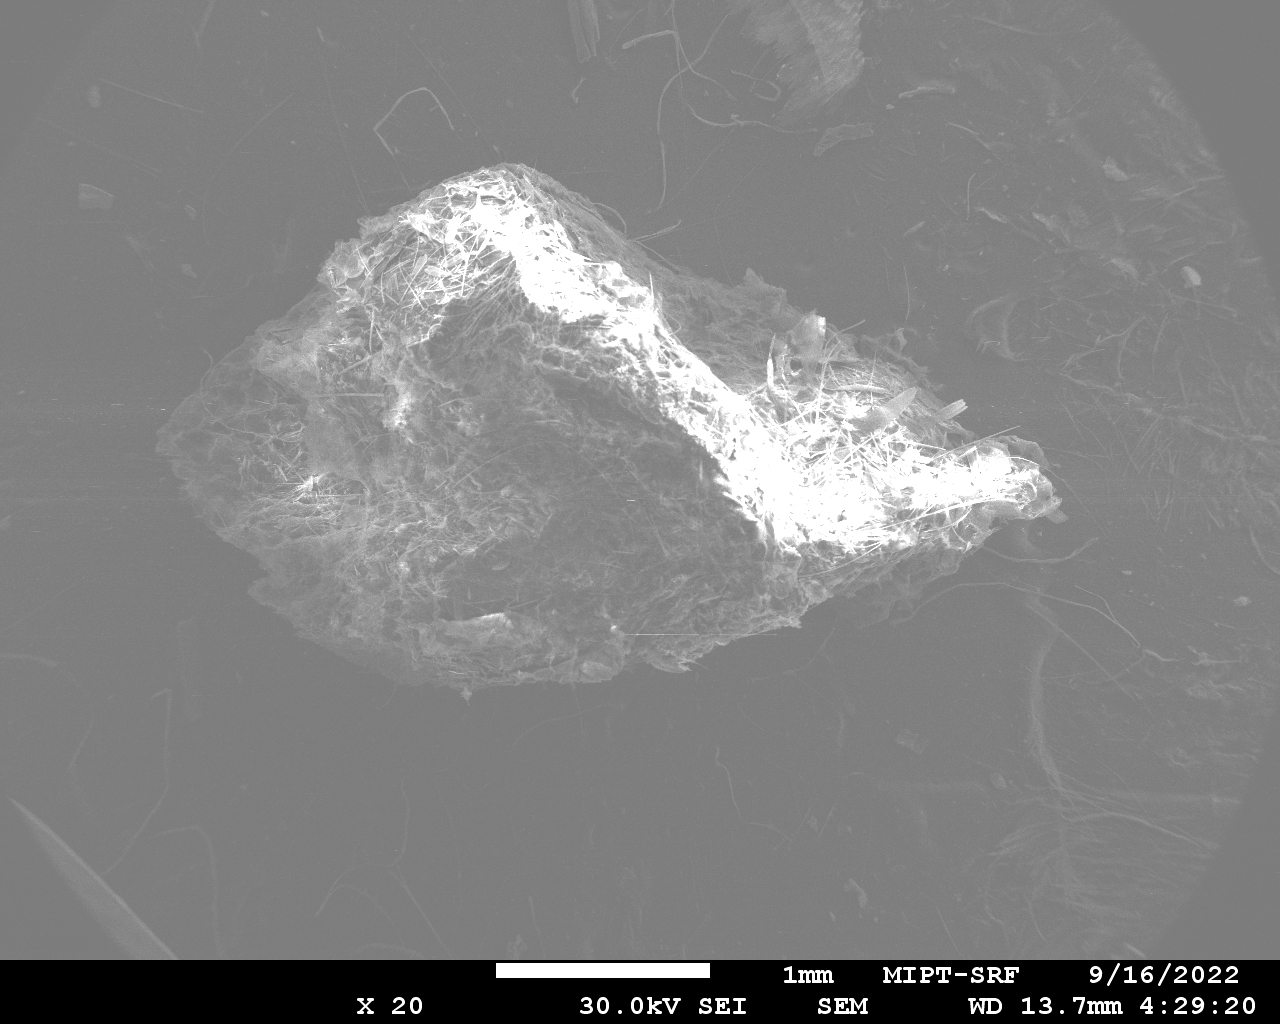
\includegraphics[width=\textwidth]{Foam001.jpg}
\vspace{-2em}
\center{(а)}
\end{minipage}
\begin{minipage}{0.49\textwidth}
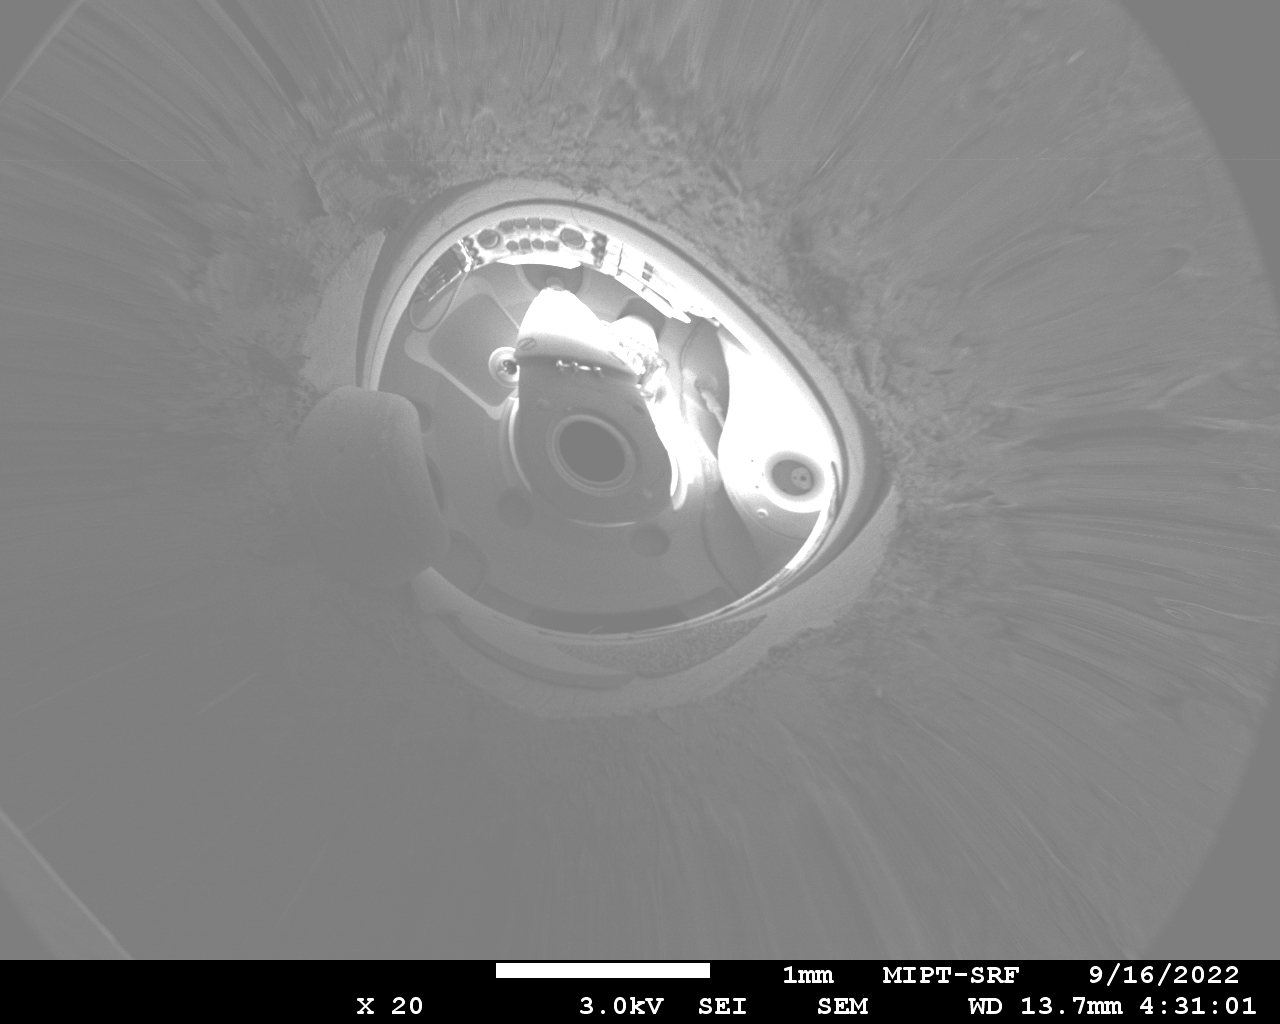
\includegraphics[width=\textwidth]{Foam002.jpg}
\vspace{-2em}
\center{(б)}
\end{minipage}
\begin{minipage}{0.49\textwidth}
\vspace{0.5em}
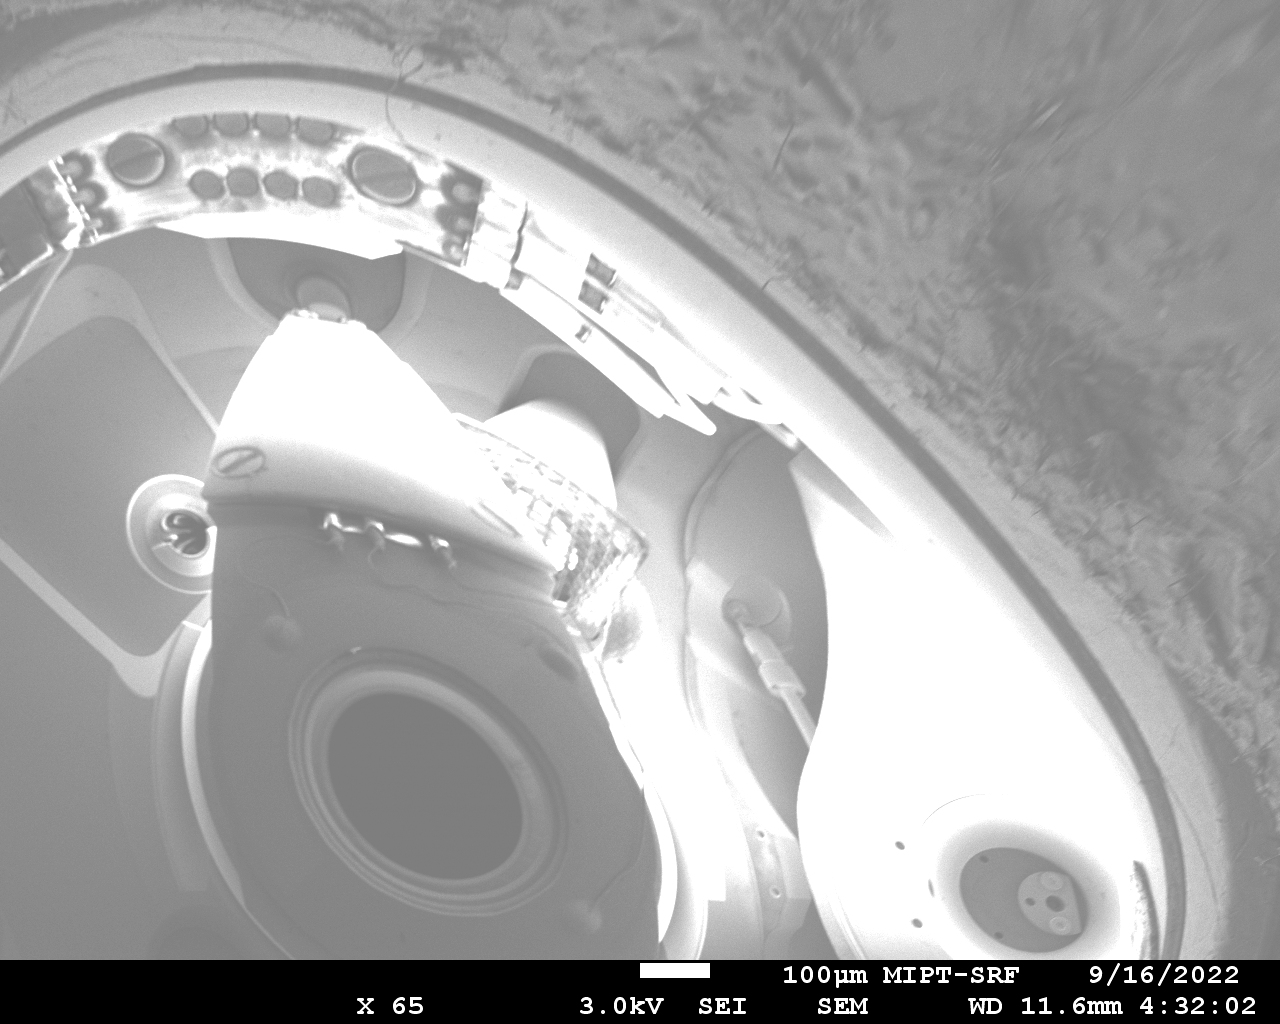
\includegraphics[width=\textwidth]{Foam003.jpg}
\vspace{-2em}
\center{(в)}
\end{minipage}
\begin{minipage}{0.49\textwidth}
\vspace{0.5em}
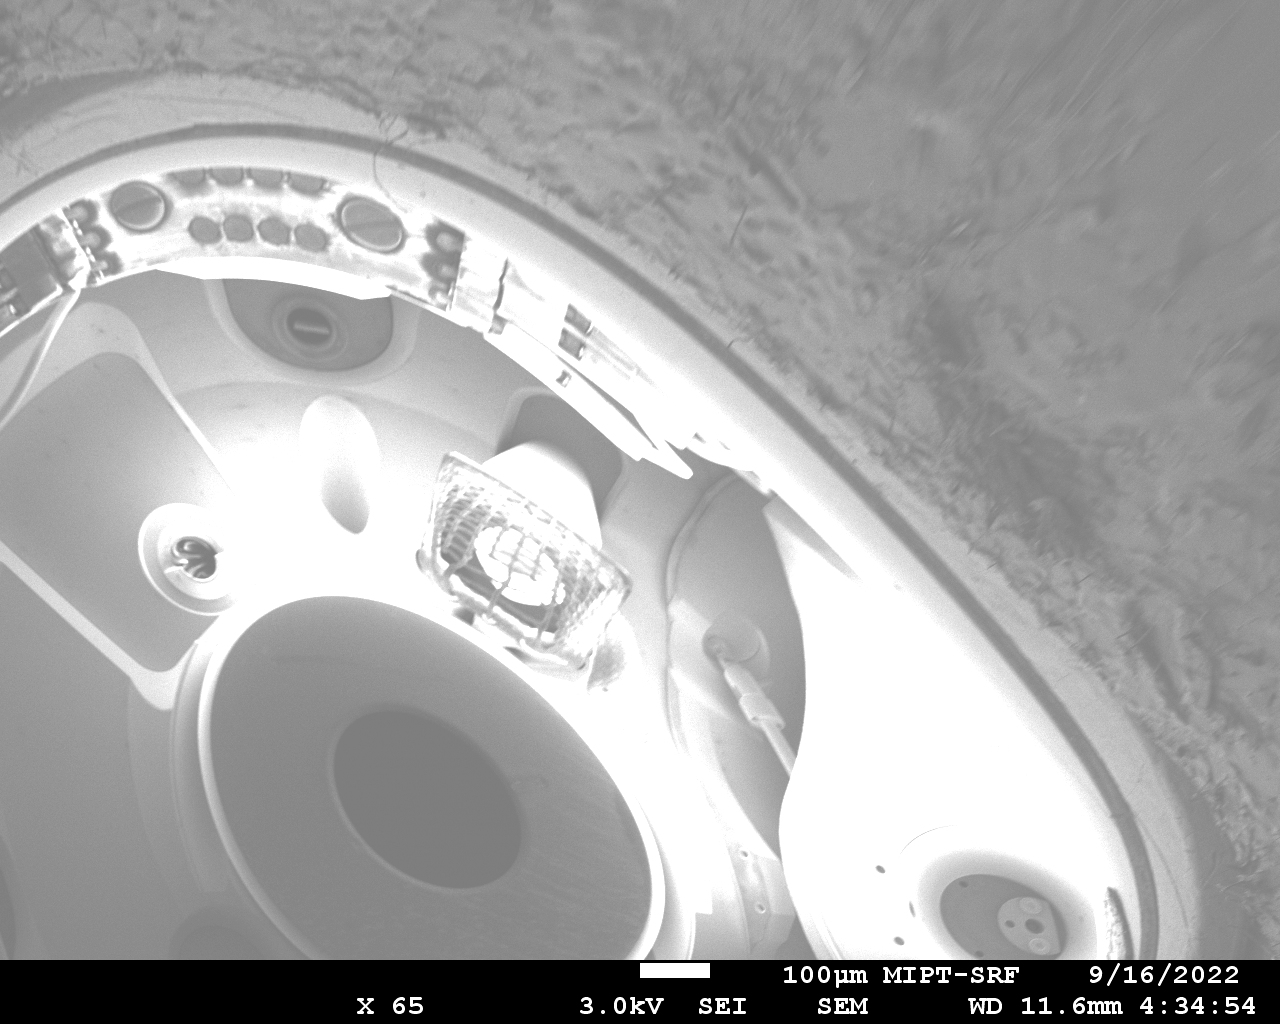
\includegraphics[width=\textwidth]{Foam004.jpg}
\vspace{-2em}
\center{(г)}
\end{minipage}
\caption{Изображение полученное при рассмотрении в РЭМ заряженного диэлектрика}
\label{fig:reflect}
\end{figure}

\end{document}
